% !TEX root = main.tex
% !TeX spellcheck = en_US

\section{Evaluation}\label{sec:eval}
We compare the communication complexity (informally, the ``bandwidth'') of \saik, \protITK and the \protCMPKE
protocol from \cite{hashimoto2021cmpke}. For the sake of this comparison (and to simplify the description), one
can think of \protCMPKE as a protocol similar to \saik but where the ratchet tree is an $N$-ary tree of height $1$, where $N$ is the number of group members.
This means that \protCMPKE only needs single-message multi-recipient PKE, \mPKE (which is a special case of mmPKE).
To make a fair comparison, we instantiate \protCMPKE with the same DH-based \mPKE as \saik
instead of the less efficient but post-quantum secure \mPKE
given in \cite{hashimoto2021cmpke}.

%Plots for sender and receiver bandwidth are in \cref{fig:plots}. All values are calculated and we provide the used
%formulas in \cref{tab:bandwidth}.

\paragraph{Methodology.}
More precisely, we break down the communication complexity into the \emph{sender bandwidth}, i.e., the size of a packet uploaded to the server, and the \emph{receiver bandwidth}, i.e., the size of a (personalized) packet downloaded by a single receiver.

We note that for \saik, the receiver bandwidth (i.e. the number of fields in the packet) differs depending on \emph{the position of the receiver in the ratchet tree}, relative to the sender. (The reason is that only public keys on the path from the sender to the lowest common ancestor in the ratchet tree need to be downloaded.) Therefore, for all protocols we compare the average receiver bandwidth over all members of the group. (For \protITK and \protCMPKE it makes no difference.)

Another difficulty in making a meaningful comparison is that for \saik and \protITK the bandwidth can vary quite
significantly depending on \emph{the execution history}. The reason is that add and remove operations may destroy the
good properties of the ratchet tree, increasing the number of recipients to which some message must be encrypted. In the
best case, there are only $\log(N)$ recipients. Roughly, this happens when the ratchet has no blank nodes or unmerged
leaves, as depicted in \cref{fig:tree-full}. However, in the worst case there can be $N$ recipients. This happens e.g. when all
non-leaf nodes are blank; see \cref{fig:tree-blank}. In general, the number of recipients can be anything in between;
see \cref{fig:tree-mixed}.

\begin{figure}[!tb]
  \centering
  \begin{tikzpicture}[->,>=stealth',level/.style={sibling distance = 6cm/#1,
      level distance = 1.5cm},scale=0.6, transform shape,
    treenode/.style = {circle, draw=black, align=center, minimum size=.9cm}]
    
    \node[treenode](root){$\mmpkepk_{\text{root}}$}
    child{
      node[treenode]{$\mmpkepk_{0}$}
      child{
        node[treenode]{$\mmpkepk_{00}$}
        child{
          node[treenode]{$\mmpkepk'_{1}$}
        }
        child{
          node[treenode]{$\mmpkepk'_{2}$}
        }       
      }
      child{
        node[treenode]{$\mmpkepk_{01}$}
        child{
          node[treenode]{$\mmpkepk'_{3}$}
        }
        child{
          node[treenode]{$\mmpkepk'_{4}$}
        }
      }
    }
    child{
      node[treenode]{$\mmpkepk_{1}$}
      child{
        node[treenode]{$\mmpkepk_{10}$}
        child{
          node[treenode]{$\mmpkepk'_{5}$}
        }
        child{
          node[treenode]{$\mmpkepk'_{6}$}
        }       
      }
      child{
        node[treenode]{$\mmpkepk_{11}$}
        child{
          node[treenode]{$\mmpkepk'_{7}$}
        }
        child{
          node[treenode]{$\mmpkepk'_{8}$}
        }
      }
    };
  \end{tikzpicture}
  \caption{A ratchet tree for \saik or \protITK without blanks or unmerged leaves.}
  \label{fig:tree-full}
\end{figure}


\begin{figure}[!tb]
  \centering
    \begin{tikzpicture}[->,>=stealth',level/.style={sibling distance = 6cm/#1,
      level distance = 1.5cm},scale=0.6, transform shape,
    treenode/.style = {circle, draw=black, align=center, minimum size=.9cm}]

    \node[treenode](root){$\mmpkepk_{\text{root}}$}
    child{
      node[treenode]{$\bot$}
      child{
        node[treenode]{$\bot$}
        child{
          node[treenode]{$\mmpkepk_{1}$}
        }
        child{
          node[treenode]{$\mmpkepk_{2}$}
        }       
      }
      child{
        node[treenode]{$\bot$}
        child{
          node[treenode]{$\mmpkepk_{3}$}
        }
        child{
          node[treenode]{$\mmpkepk_{4}$}
        }
      }
    }
    child{
      node[treenode]{$\bot$}
      child{
        node[treenode]{$\bot$}
        child{
          node[treenode]{$\mmpkepk_{5}$}
        }
        child{
          node[treenode]{$\mmpkepk_{6}$}
        }       
      }
      child{
        node[treenode]{$\bot$}
        child{
          node[treenode]{$\mmpkepk_{7}$}
        }
        child{
          node[treenode]{$\mmpkepk_{8}$}
        }
      }
    };
  \end{tikzpicture}
  \caption{A ratchet tree for \saik or \protITK with all nodes blank.}
  \label{fig:tree-blank}
\end{figure}


\begin{figure}[!tb]
  \begin{tikzpicture}[->,>=stealth',level/.style={sibling distance = 6cm/#1,
      level distance = 1.5cm},scale=0.6, transform shape,
    treenode/.style = {circle, draw=black, align=center, minimum size=.9cm}]
    
    \node[treenode](root){$\mmpkepk_{\text{root}}$}
    child{
      node[treenode]{$\bot$}
      child{
        node[treenode]{$\bot$}
        child{
          node[treenode]{$\mmpkepk'_{1}$}
        }
        child{
          node[treenode]{$\mmpkepk'_{2}$}
        }       
      }
      child{
        node[treenode]{$\mmpkepk_{01}$}
        child{
          node[treenode]{$\mmpkepk'_{3}$}
        }
        child{
          node[treenode]{$\mmpkepk'_{4}$}
        }
      }
    }
    child{
      node[treenode]{$\mmpkepk_{1}$}
      child{
        node[treenode]{$\bot$}
        child{
          node[treenode]{$\mmpkepk'_{5}$}
        }
        child{
          node[treenode]{$\mmpkepk'_{6}$}
        }       
      }
      child{
        node[treenode]{$\mmpkepk_{11}$}
        child{
          node[treenode]{$\mmpkepk'_{7}$}
        }
        child{
          node[treenode]{$\mmpkepk'_{8}$}
        }
      }
    };
  \end{tikzpicture}
  \caption{A tree with some blank and non-blank nodes. Here, sender bandwidth depends on the position in the
    tree. For example, a packet by the leftmost leaf would contain 5 ciphertexts, while the rightmost leaf would require 6.}
  \label{fig:tree-mixed}
\end{figure}

%%% Local Variables:
%%% mode: latex
%%% TeX-master: "main"
%%% End:


Comparing the average over all execution histories would not be meaningful, since the probability of a given execution depends on the setting such as user and administrator behavior and general
governing policies, which is outside the
scope of this work. Indeed, it is an important topic of future research to
better understand which kinds of policies governing when and which parties
initiate CGKA operations lead to more bandwidth efficient executions for
realistic deployments. Therefore, we compare the minimum and maximum bandwidth over all possible execution histories.


%The packet size of \protCMPKE depends only the current group size. However,
%for both binary tree-based protocols (i.e. \saik and \protITK), the size of a
%packet sent (i.e. the number of fields it contains) can vary quite
%significantly depending on the session history and sender. This is due to the fact some operations will blank nodes in
%the ratchet tree, which increases the number of encryptions. Consequently, the
%plots consist of regions rather than lines, where the upper bound is for a completely blank tree and the lower bound for
%a tree without any blanks. We refer to these two cases as best-case and worst-case respectively. Still, the protocols have
%identical behavior in this regard, i.e. for a given group size $N$, history of
%past CGKA operations and a next operation the number and position of blanks in the tree is identical and therefore the
%number of fields in the resulting (full) packet is the same for both protocols. What does change are
%the size of some of the fields and, of course, which ones are downloaded by
%the receiver.
%(So for example, if the next packet sent for \saik is at the bottom of
%\saik's indicated size range then same holds for \protITK; namely its next
%packet size will also be at the bottom of its size range.)
%
%Additionally, in \saik, the size of the downloaded package differs depending on the position of the receiver in the tree
%relative to the sender, as only public keys on the path from the sender to the lowest common ancestor in the ratchet
%tree need to be downloaded. Therefore, we consider the \emph{average} receiver bandwidth for \saik (in \protITK and
%\protCMPKE, all receiver packages have the same size, so this doesn't matter).

%We remark that determining ``average'' or ``expected'' numbers and positions of blanks in the ratchet tree would require
%first fixing many setting-dependent aspects of an execution such as user and administrator behavior and general
%governing policies, which is outside the
%scope of this work. Indeed, it is an important topic of future research to
%better understand which kinds of policies governing when and which parties
%initiate CGKA operations lead to more bandwidth efficient executions for
%realistic deployments.
%Note that these considerations do not apply to \protCMPKE, as it doesn't arrange its group members as a tree, so it
%doesn't have to deal with blank nodes.
%\mnote{we never said in this section that O(N) complexity is a result of
%blank nodes so it may be confusing for people who jump here from the intro. I
%would just say this but no strong opinions.}


\newcommand{\ctxSize}{\variable{Ctx}}
\newcommand{\mCtxSize}{\variable{mCtx}}
\newcommand{\pkSize}{\variable{Pk}}
\begin{figure*}[!t]
	\begin{minipage}[t]{\textwidth}\centering
	\begin{tabulary}{\linewidth}{|l|l|l|l|l|}
		\hline
		\multicolumn{2}{|c|}{}& \protITK & \saik & \protCMPKE \\
		\hline
		\multirow{2}{*}{Sender} 
		& best case & $\log(N)\cdot (\pkSize + \ctxSize)$ & $\log(N) \cdot \pkSize + \mCtxSize(\log(N))$ & $\pkSize + \mCtxSize(N)$ \\\cline{2-5}
		& worst case & $\log(N)\cdot\pkSize + N\cdot \ctxSize$ & $\log(N) \cdot \mmpkepk + \mCtxSize(N)$ & $\pkSize + \mCtxSize(N)$ \\\hline
		\multirow{2}{*}{(Average) receiver} 
		& best case & $\log(N)\cdot (\pkSize + \ctxSize)$  & $\log(N) \cdot \pkSize + \ctxSize$  & $\pkSize + \ctxSize$ \\\cline{2-5}
		& worst case &  $\log(N)\cdot\pkSize + N\cdot \ctxSize$ & $\log(N) \cdot \pkSize + \ctxSize$  & $\pkSize + \ctxSize$ \\
		\hline
	\end{tabulary}
	\caption{Sender and receiver bandwidth for a group of size $N$ expressed as the number of ciphertexts and public keys included in the packet (apart from this, packets include only a constant-size header).
		$\pkSize$ denotes the size of a public key (the same for PKE and mmPKE). $\mCtxSize(X)$ denotes the size of an mmPKE multi-recipient ciphertext with overall number of receivers $X$. Note that for the DH-based construction $X$ fully determines the size (i.e., it is not affected by who gets which message). $\ctxSize$ denotes the size of a PKE ciphertext, equal to the size of an individual ciphertext in the DH-based construction.
	}
	\label{tab:bandwidth1}
\end{minipage}
  \begin{minipage}[t]{.48\textwidth}
	\begin{minipage}[t]{\linewidth}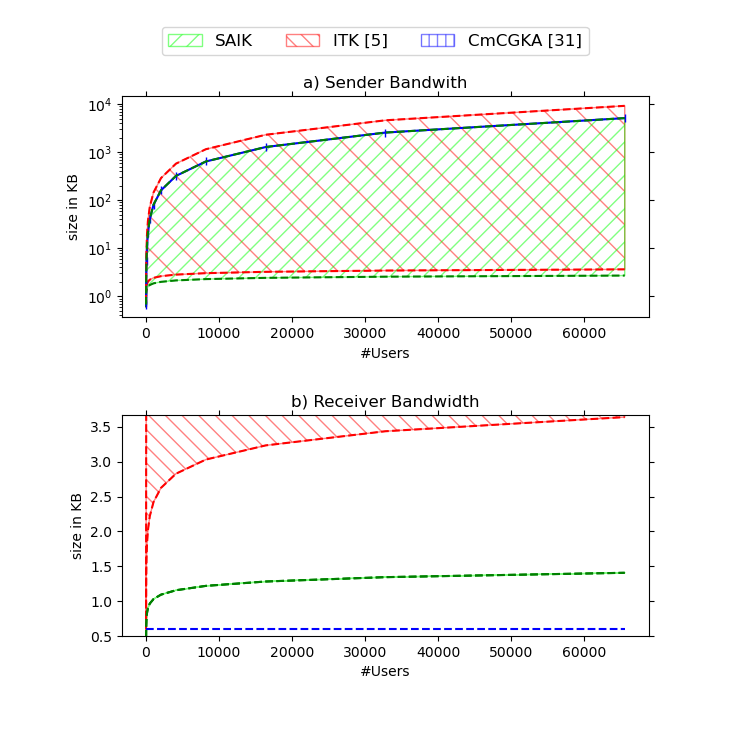
\includegraphics[width=\linewidth]{../plots/Final_Figures_Avg}\end{minipage}\vspace*{-1cm}
	\caption{Bandwidth comparison of \saik, \protITK and \protCMPKE (instantiated with 256-bit
		security). Lower lines denote the best case execution history, while upper lines denote the
		worst case. All other possible cases are marked as the regions between the lines. Plot (a) shows the sender bandwidth on a \emph{log scale} and plot
		(b) shows average individual receiver bandwidth on a \emph{linear scale}. Note that in the first plot, the lines for worst-case \saik and
		all-case \protCMPKE coincide.
		%Sender and receiver bandwidth for a group of size $N$ expressed as the (approximate) number of group elements.
	}
	\label{tab:plots}
  \end{minipage}
  \hfill
  \begin{minipage}[t]{.48\textwidth}
    \centering\vspace*{-8cm}
    \begin{minipage}[t]{\linewidth}
    	\begin{tabulary}{\linewidth}{|l|l|l|l|l|}
    		\hline
    		\multicolumn{2}{|c|}{}& \protITK & \saik & \protCMPKE \\
    		\hline
    		\multirow{2}{*}{Sender} 
    		& best case & $3\log(N)$ & $2\log(N)$ & $N$ \\\cline{2-5}
    		& worst case &$2N$ & $N$ & $N$ \\\hline
    		\multirow{2}{*}{\parbox{2cm}{(Average)\\receiver}} 
    		& best case & $3\log(N)$ & $\log(N)$&  $3$ \\\cline{2-5}
    		& worst case & $2N$ & $\log(N)$ & $3$ \\
    		\hline
    	\end{tabulary}
    \caption{
    	Sender and receiver bandwidth for a group of size $N$ expressed as the (approximate) number of group elements.
    }\cref{fig:bandwidth2}
  \end{minipage}


  \begin{minipage}[t]{\linewidth}\centering
    \begin{tabulary}{\linewidth}{|l|r|}
      \hline
      & Bitsize \\
      \hline
      Group element & 512 \\
      \hline
      Hash & 512 \\
      \hline
      Signature & 1024 \\
      \hline
      Header & 17944 \\
      \hline
      \pkSize & 512 \\
      \hline
      \ctxSize & 1152 \\
      \hline
      $\mCtxSize(N)$ & $512 + N \cdot 640$ \\
      \hline
    \end{tabulary}
    \caption{Bitsizes used to generate \cref{fig:plots}. The header consists of the sender's id, the epoch id and some
      authenticated data required by the protocol. The individual ciphertexts consist of a group element and an AEAD
      encryption, while the \mPKE ciphertext all share the same group element. The header contains signatures, tags,
      epoch and sender identifier as well as a key package. The latter makes up the bulk of the header, as it contains
      credentials, more public keys and some application data. Our estimation is based on MLS.}
    \label{tab:bitsizes}
  \end{minipage}
  \end{minipage}
\end{figure*}
\paragraph{Results.}
We estimated the bandwidth for all protocols using the formulas in \cref{tab:bandwidth1,tab:bandwidth2} with bit lengths
as indicated in \cref{tab:bitsizes}. This is further visualized in \cref{fig:plots} for growing group sizes $N$.
%
% Further, \cref{fig:plots} shows how the concrete bandwidth, for the group {\color{red} help :) } ) of the three protocols scales as the group size $N$ grows.
%
We highlight some interesting observations. % features of the plots. %For concreteness, we fix $N = 10K$ users.

For senders, \saik is always at least as good as the other protocols. First, it requires between $84\%$ and only $55\%$
of the bandwidth of \protITK (due to the use of mmPKE). Second, the bandwidth of \protCMPKE is the same as the
worst-case (depending on the execution history) bandwidth of \saik. In the best case, however, \saik needs as little as
$0.52\%$ of the bandwidth, e.g. in a group of $10K$ members it can save as much as $\sim 779$KB out of total
$783$KB.


% Even for senders,
%\saik requires between $83\%$ to just $55\%$ of the bandwidth of \protITK due to
%\saik's use of \mmPKE. While receiver bandwidth is constant for \protCMPKE,
%its sender bandwidth is always as bad as the worst case for \saik. 
% In the
%best case, \saik needs as little as $0.45\%$ of the bandwidth, e.g. in a
%group of $10K$ members it can save as much as $\sim 780$KB out of total
%$783$KB.


% ITK vs SAIK, sender : 122% -> 179%
% ITK vs ITKI, sender : 72% -> 52%
% SAIK-Huffman vs ITK, 1-receiver : % improvement grows with group size. Best case from 165% -> 200K%.
% Huffman vs Merkel, cumulative server : % improve is 0% -> 5% (though proof sizes improve by up to %50)

For receivers, \protITK is \emph{overwhelmingly} worse than \saik and \protCMPKE. For
example, \saik receivers (on average) need between $62\%$ (best-case execution) to about $.2\%$ (worst-case execution)
of \protITK's. On the other hand, \protCMPKE is (unsurprisingly) the best for receivers.  \saik requires up to $126\%$
of \protCMPKE's bandwidth, i.e. an increase of $\sim 0.62$KB from $\sim 2.4$KB for a group of $10K$ members.

%On the receiver side, \protITK is \emph{overwhelmingly} worse than \saik. For
%example, \saik receivers (on average) need between $60\%$(full tree) to about $.05\%$(blank tree) of \protITK's
%bandwidth. On the other hand, the receiver side has constant bandwidth for
%\protCMPKE. \saik requires up to $137\%$ of \protCMPKE's bandwidth, i.e. an
%increase of $\sim 0.75$KB from $\sim 2$KB.

\paragraph{Server computation.}
Lastly, we consider the server-side computation for \saik and \protCMPKE. In \protCMPKE, the server only picks the
$i$-th \mPKE ciphertext for the $i$-th user and forwards all common data. For \saik, we can consider two possibilities:
Either the server keeps track of the shape of the ratchet tree (which it can do based on the header data sent in all
packages) and computes the lowest common ancestor of sender and receiver in the tree, computes its resolution and then
forwards the corresponding ciphertext and public keys. This takes at most logarithmic time in the size of the
group (however, no expensive public-key operations are required). Alternatively, the user can compute its indices in the
tree and send them to the server, reducing the server computation to effectively the same as in \protCMPKE at the cost
of an additional round of communication.

% {\color{red} remove this?}
% \dnote{Yes, especially if one of the reviewers really is an author of 31.}
% We note that a CGKA with a similar efficiency profile to \protCMPKE can be
% constructed directly using 2-party secure messaging channels between each
% pair of group members (implemented e.g. by the double ratchet).
% %from a pairwise secure channels, e.g. via the
% %Signal double ratchet.
% To create a new epoch, a sender samples a fresh commit secret and sends it
% (along with fields identifying the group, epoch and the desired group
% operation) to all group members. The commit secret is then used analogous to
% \protITK: it is hashed together with the previous init secret (as well as
% context information) to derive a new epochs key schedule. \protCMPKE doesn't
% use pairwise secure channels but instead redraws abstraction boundaries to
% enable the use of multi-recipient PKE (\mPKE). This allows them to be roughly
% twice as efficient as the outlined protocol.


%\begin{table*}[ht]
%	\begin{tabulary}{\linewidth}{C|ccc}
%		Abstract & \protITK & \saik & \protCMPKE \\
%		\hline
%		Sender Full Tree & $\log(N)*(\mmpkepk + \pathSecCtxt)$ & $\log(N) * \mmpkepk + \mmpkeCtxt(\log(N))$ & $\mmpkeCtxt(N)
%		+ \mmpkepk$ \\
%		Sender Empty Tree & $\log(N)*\mmpkepk + N* \pathSecCtxt$ & $\log(N) * \mmpkepk + \mmpkeCtxt(N)$ & $\mmpkeCtxt(N) +
%		\mmpkepk$ \\
%		Receiver Avg. Full Tree & $\log(N)*(\mmpkepk + \pathSecCtxt)$ & \multirow{2}*{$\log(N) * \mmpkepk + \pathSecCtxt$}  & \multirow{2}*{$\mmpkepk + \pathSecCtxt$}  \\
%		Receiver Avg. Empty Tree & $\log(N)*\mmpkepk + N* \pathSecCtxt$ &   &  \\
%		\hline
%		\hline
%		Concrete & & & \\ 
%		\hline
%		Sender Full Tree & $\sim 3\log(N)*\Grp$ & $\sim 2\log(N)*\Grp$ & $\sim N*\Grp$ \\
%		Sender Empty Tree & $\sim2N*\Grp$ & $\sim N*\Grp$ & $\sim N*\Grp$ \\
%		Receiver Avg. Full Tree & $\sim 3\log(N)*\Grp$ & \multirow{2}*{$\sim \log(N)*\Grp$}  & \multirow{2}*{$3*\Grp$} \\
%		Receiver Avg. Empty Tree & $\sim 2N*\Grp$ &  &  \\
%	\end{tabulary}
%	\caption{Formula for server and (average) receiver bandwidth for full and empty trees. The first half of the table
%		denotes the abstract bandwidth relative to the used primitives, while the latter half assumes that everything is
%		instantiated over a common prime-order group $\grp$ with the size of a group element denoted by $\Grp$. We assume
%		\saik and \protCMPKE both use the $\mmPKE$ described in \cref{sec:mmpke} and ignore common constants such as signatures and headers.}
%	\label{tab:bandwidth}
%\end{table*}
%%% Local Variables:
%%% mode: latex
%%% TeX-master: "main"
%%% End:
